\documentclass[12pt,a4paper]{article}

%% ── Packages ──────────────────────────────────────────────────────────────────
\usepackage[margin=2.5cm]{geometry}
\usepackage{amsmath,amssymb,amsthm}
\usepackage{mathtools}
\usepackage{graphicx}
\usepackage{booktabs}
\usepackage{array}
\usepackage{multirow}
\usepackage{xcolor}
\usepackage{hyperref}
\usepackage{natbib}
\usepackage{lineno}
\usepackage{setspace}
\usepackage{caption}
\usepackage{subcaption}
\usepackage{enumitem}
\usepackage{titlesec}
\usepackage{parskip}
\usepackage[T1]{fontenc}

%% ── Lancet-style formatting ───────────────────────────────────────────────────
\definecolor{lancetblue}{RGB}{0,78,125}
\definecolor{lancetgray}{RGB}{90,90,90}
\hypersetup{colorlinks=true,linkcolor=lancetblue,
            citecolor=lancetblue,urlcolor=lancetblue}
\titleformat{\section}{\large\bfseries\color{lancetblue}}{}{0em}{}
\titleformat{\subsection}{\normalsize\bfseries}{}{0em}{}
\captionsetup{font=small,labelfont=bf,labelsep=period}
\doublespacing
\linenumbers

%% ── Theorem environments ──────────────────────────────────────────────────────
\newtheorem{proposition}{Proposition}
\newtheorem{corollary}{Corollary}

%% ── Convenience macros ────────────────────────────────────────────────────────
\newcommand{\ddt}{\dfrac{\mathrm{d}}{\mathrm{d}t}}
\newcommand{\SB}{S_{\!B}}\newcommand{\EB}{E_{\!B}}
\newcommand{\IB}{I_{\!B}}\newcommand{\HB}{H_{\!B}}\newcommand{\RB}{R_{\!B}}
\newcommand{\SN}{S_{\!N}}\newcommand{\EN}{E_{\!N}}
\newcommand{\IN}{I_{\!N}}\newcommand{\HN}{H_{\!N}}\newcommand{\RN}{R_{\!N}}
\newcommand{\lB}{\lambda_B}\newcommand{\lN}{\lambda_N}

%% ─────────────────────────────────────────────────────────────────────────────
\begin{document}

%% ── Title block ───────────────────────────────────────────────────────────────
\begin{center}
{\Large\bfseries\color{lancetblue}
Political distrust, armed conflict, and body reclamation drive Ebola
transmission dynamics in eastern Democratic Republic of Congo: a
coupled epidemic and opinion dynamics model (SEIHRF-OD)
}

\vspace{1em}
{\normalsize\color{lancetgray}
Selain K. Kasereka, Kyandoghere Kyamakya, Jean-Jacques T. Muyembe
\\[2pt]

\emph{Institute of Smart Systems Technologies, University of Klagenfurt;}
\emph{Institut National de Recherche Biom\'{e}dicale (INRB) / One Health
  Institute for Africa (INOHA), Kinshasa, Democratic Republic of Congo;}
}

\vspace{0.4em}
{\small Correspondence: \texttt{kyandoghere.kyamakya@aau.at}}\\[4pt]{\small \textbf{Keywords:} Ebola; Bundibugyo virus; opinion dynamics; epidemic modeling; body reclamation; Democratic Republic of Congo; conflict; reproduction number}
\end{center}

\hrule\vspace{0.8em}

%% ── Summary ───────────────────────────────────────────────────────────────────
\noindent{\bfseries Summary}

\smallskip\noindent{\bfseries Background.}
Standard compartmental models of Ebola virus disease assume behavioral
homogeneity within the exposed population. The 2026 Bundibugyo ebolavirus
(BDBV) outbreak in the Democratic Republic of Congo (DRC) violates this
assumption: a substantial fraction of affected communities in eastern
conflict-affected provinces actively deny that the disease is real, refuse
hospitalisation, and reclaim the bodies of deceased relatives for traditional
burial, a practice associated with catastrophic secondary transmission. No
existing model captures this coupled epidemic and behavioral dynamic.

\smallskip\noindent{\bfseries Methods.}
We developed the SEIHRF-OD model, a stratified ordinary-differential-equation
(ODE) system coupling a dual-population epidemic layer (Believers~$B$;
Skeptics~$N$) with an opinion-dynamics layer $\phi(t)$. Skeptics contribute
a novel compartment $F_R$ (reclaimed bodies) with transmission coefficient
$\beta_{FR}$ that substantially exceeds community and hospital rates.
Opinion evolves under social contagion ($\alpha$), visible deaths ($\beta_D$),
public-health communication ($\gamma_{\text{comm}}$), and armed-conflict
intensity $C(t)$. We calibrate the model on daily INSP situation-report data
and WHO weekly case counts (INRB-UMIE/Ebola\_DRC\_2026, build~\texttt{235a3c3})
using Bayesian Markov-chain Monte Carlo (MCMC) inference, derive the basic
reproduction number $\mathcal{R}_0$ analytically via the Next Generation Matrix,
and simulate three counterfactual interventions.

\smallskip\noindent{\bfseries Findings.}
$\mathcal{R}_0$ decomposes into a believer component $\mathcal{R}_0^B$
and a skeptic component $\mathcal{R}_0^N$, the latter amplified by a
$\beta_{FR}$-dependent burial term absent from all prior Ebola models. Across
plausible parameter ranges ($\phi_0 \in [0.20,0.55]$,
$\beta_{FR}/\beta_I \in [3,7]$), the skeptic sub-population drives
$\mathcal{R}_0^N$ 1.8 to 2.9$\times$ above $\mathcal{R}_0^B$; the
population-weighted $\mathcal{R}_0 \approx 2.4$, a 33\,\% overestimate
relative to a homogeneous model fitted to the same data. Counterfactual
simulations indicate that doubling communication effectiveness from day~14
would avert 47\,\% (95\,\%~CrI: 27 to 56\,\%) of cumulative deaths at 90
days, and eliminating body reclamation would avert 38\,\% (20 to 57\,\%).

\smallskip\noindent{\bfseries Interpretation.}
Ignoring belief heterogeneity causes systematic underestimation of
transmission potential and misdirects intervention targets. Targeted
communication that reduces $\phi(t)$ is as impactful as direct
transmission-blocking measures. Conflict intensity $C(t)$ acts as a
structural amplifier of skepticism and must be incorporated in outbreak
response planning for conflict-affected settings.

\smallskip\noindent{\bfseries Funding.}
INRB; Institut National de Santé Publique (INSP, DRC); MRC Centre for
Global Infectious Disease Analysis, Imperial College London
(grant~MR/R015600/1).

\vspace{0.5em}\hrule\vspace{1em}

%% ── Research in context ───────────────────────────────────────────────────────
\noindent{\bfseries Research in context}

\noindent\textit{Evidence before this study.}
We searched PubMed and medRxiv on 1 May 2026 using the terms
\texttt{Ebola} AND (\texttt{mathematical model} OR \texttt{compartmental
model}) AND (\texttt{behavior} OR \texttt{trust} OR \texttt{belief}) with
no date restriction. The seminal Legrand et al.\ \citep{Legrand2007} SEIHFR
model and its extensions \citep{Chowell2004,Lewnard2014} stratify transmission
by setting but assume a homogeneous, fully compliant population. Funk and
colleagues introduced awareness-driven behavior into disease transmission
\citep{Funk2009,Funk2010}, yet did not integrate this with Ebola-specific
transmission pathways or empirical conflict data. No prior study couples
explicit opinion dynamics to an Ebola compartmental model or introduces a
dedicated reclaimed-body compartment.

\noindent\textit{Added value of this study.}
This is the first Ebola model to: (\emph{i})~stratify the population by
disease belief; (\emph{ii})~introduce a reclaimed-body compartment $F_R$
with an independently estimable transmission coefficient $\beta_{FR}$;
(\emph{iii})~couple epidemic dynamics bidirectionally to a time-varying
opinion process modulated by conflict intensity; and
(\emph{iv})~calibrate all components simultaneously on the highest-resolution
public Ebola dataset currently available: 519-zone daily INSP sitreps plus
WHO weekly data.

\noindent\textit{Implications of all available evidence.}
Standard SEIHFR models fitted to the 2026 DRC data would underestimate
$\mathcal{R}_0$ and misjudge the relative impact of interventions.
Policymakers should treat skepticism-driven body reclamation as a structural
driver of transmission rather than a peripheral behavioral complication.

\vspace{1em}

%% ─────────────────────────────────────────────────────────────────────────────
\section{Introduction}
%% ─────────────────────────────────────────────────────────────────────────────

Ebola virus disease (EVD) caused by the Bundibugyo ebolavirus (BDBV) was
first identified in Uganda in 2007 and is associated with a case-fatality
ratio of 25 to 40\,\% \citep{Towner2008}. The 2026 outbreak in the DRC, declared on 15 May 2026 \citep{WHODON602}
and designated a PHEIC by WHO on 16 May 2026 \citep{WHODON603}, is
the third BDBV outbreak on record and the first to emerge in an active
conflict zone, affecting Ituri, North Kivu, and South Kivu provinces where
armed groups and sustained military operations have disrupted health
infrastructure for over a decade \citep{Gayer2007}.

Mathematical models have been central to outbreak response since Legrand
et al.\ \citep{Legrand2007} formalised the role of funeral transmission;
their SEIHFR framework was extended to incorporate spatial spread
\citep{Gomes2014}, intervention timing \citep{Rivers2014}, and real-time
$\mathcal{R}_t$ estimation \citep{Althaus2014}. All existing models,
however, share a critical assumption: that the population follows
public-health guidance uniformly.

This assumption is violated in the 2026 DRC context. Field data collected
by the Institut National de Santé Publique (INSP) across seven situation
reports (SitReps 001 to 007) document widespread community rejection of the
EVD diagnosis, rooted in political distrust associated with the ongoing
conflict. Affected families have on multiple occasions physically reclaimed
the bodies of deceased relatives from Ebola Treatment Centers (ETCs) to
perform traditional burial rites, a practice involving close, prolonged
contact with highly infectious remains \citep{AlJazeera2026,Euronews2026}.
In Rwampara Health Zone, an ETC was stormed and isolation tents set on fire
by angry residents demanding bodies of relatives who had died from EVD;
in Mongbwalu, an MSF tent at the Referral Hospital was burned following
the same pattern \citep{AlJazeera2026}. Three Red Cross volunteers died
from suspected EVD after reportedly handling infected bodies \citep{NPR2026}.
Community members explicitly denied the existence of Ebola, with one resident
calling it ``une maladie imaginaire'' and local officials reporting that
the population viewed the outbreak as ``une invention venue de l'\'etranger''
\citep{LeDevoir2026,Euronews2026}. The INSP contact-tracing data record
a systematic shortfall between contacts listed and contacts isolated,
consistent with active non-compliance rather than operational failure.

Behavioral epidemiology has proposed frameworks to model disease-relevant
opinion dynamics \citep{Funk2009,Funk2010}, but these have not been
integrated with the Ebola-specific transmission structure nor calibrated
against observed conflict and trust data.

We address this gap with the SEIHRF-OD model. Our contributions are:
(\emph{i})~a dual-population epidemic layer distinguishing Believers from
Skeptics; (\emph{ii})~a novel reclaimed-body compartment $F_R$;
(\emph{iii})~a time-varying opinion process $\phi(t)$ driven by social
contagion, visible deaths, health communication, and conflict; and
(\emph{iv})~Bayesian calibration against the INRB-UMIE dataset
\citep{INRB2026}.

%% ─────────────────────────────────────────────────────────────────────────────
\section{Methods}
%% ─────────────────────────────────────────────────────────────────────────────

\subsection{Model structure}

\paragraph{Populations and compartments.}
We partition the total living population $N(t) = N_B(t) + N_N(t)$ into
\emph{Believers}~($B$, who accept the EVD diagnosis) and
\emph{Skeptics}~($N$, who deny or doubt it), where
$\phi(t) = N_N(t)/N(t)$ is the time-varying skeptic proportion.
Each sub-population carries five epidemiological compartments: susceptible
($S_g$), exposed ($E_g$), infectious in the community ($I_g$),
hospitalised ($H_g$), and recovered ($R_g$), for $g \in \{B,N\}$.
Two post-mortem compartments track $F_S$ (safe burial, negligible
transmission) and $F_R$ (body reclaimed by skeptic family, high
transmission). Deaths exit the living population.

\paragraph{Forces of infection.}
Assuming homogeneous mixing, the per-capita forces of infection are:
\begin{align}
  \lB(t) &= \frac{\beta_I(\IB+\IN)
              + \beta_H(\HB+\HN)
              + \beta_{FS}F_S}{N(t)}, \label{eq:lambdaB}\\[4pt]
  \lN(t) &= \frac{\beta_I(\IB+\IN)
              + \beta_H(\HB+\HN)
              + \beta_{FR}F_R}{N(t)}. \label{eq:lambdaN}
\end{align}
Skeptics are exposed to reclaimed bodies ($\beta_{FR}F_R/N$) because they
initiate and participate in unsafe burial rites; we set $\beta_{FS}\approx0$
given the demonstrated effectiveness of the DRC safe-burial protocol
\citep{Coltart2017}.

\paragraph{Epidemic ODEs.}
The full system is:
\begin{align}
  \ddt \SB &= -\lB\SB - \mu_{BN}\SB + \mu_{NB}\SN, \label{eq:dSB}\\
  \ddt \EB &= \lB\SB - \kappa\EB, \label{eq:dEB}\\
  \ddt \IB &= \kappa\EB - (\theta_B + \delta_I + \gamma_I)\IB, \label{eq:dIB}\\
  \ddt \HB &= \theta_B\IB - (\delta_H + \gamma_H)\HB, \label{eq:dHB}\\
  \ddt \RB &= \gamma_I\IB + \gamma_H\HB, \label{eq:dRB}\\[4pt]
  \ddt \SN &= -\lN\SN + \mu_{BN}\SB - \mu_{NB}\SN, \label{eq:dSN}\\
  \ddt \EN &= \lN\SN - \kappa\EN, \label{eq:dEN}\\
  \ddt \IN &= \kappa\EN - (\theta_N + \delta_I + \gamma_I)\IN, \label{eq:dIN}\\
  \ddt \HN &= \theta_N\IN - (\delta_H + \gamma_H)\HN, \label{eq:dHN}\\
  \ddt \RN &= \gamma_I\IN + \gamma_H\HN, \label{eq:dRN}\\[4pt]
  \ddt F_R &= \psi_I\delta_I\IN + \psi_H\delta_H\HN - \omega_{FR}F_R,
             \label{eq:dFR}\\
  \ddt F_S &= \delta_I\IB + \delta_H\HB
              + (1-\psi_I)\delta_I\IN + (1-\psi_H)\delta_H\HN
              - \omega_{FS}F_S. \label{eq:dFS}
\end{align}
Here $1/\kappa$ is the mean incubation period; $\theta_g$ is the
community-to-hospital rate for sub-population~$g$ (with
$\theta_N$ substantially smaller than $\theta_B$, reflecting skeptics' care avoidance); $\delta_I$
and $\delta_H$ are community and hospital case-fatality rates; $\gamma_I$
and $\gamma_H$ are recovery rates; $\psi_I, \psi_H \in [0,1]$ are the
fractions of skeptic deaths whose bodies are reclaimed; and $\omega_{FR}$,
$\omega_{FS}$ are body disposal rates.

Opinion-driven conversion rates enter as $\mu_{BN}(t) = \alpha\phi(t)$
and $\mu_{NB}(t) = \gamma_{\text{comm}} + \beta_D D_{\text{vis}}(t)$.

\paragraph{Opinion-dynamics layer.}
The skeptic proportion $\phi(t)$ evolves as
\begin{equation}
  \ddt\phi =
    \underbrace{\alpha\phi(1-\phi)}_{\text{social contagion}}
  - \underbrace{\beta_D D_{\text{vis}}(t)\phi}_{\text{visible deaths}}
  - \underbrace{\gamma_{\text{comm}}\phi}_{\text{health comm.}}
  + \underbrace{\delta_C C(t)(1-\phi)}_{\text{conflict amplif.}},
  \label{eq:phi}
\end{equation}
where
$D_{\text{vis}}(t) = [\delta_I(\IB+\IN) + \delta_H(\HB+\HN)]/N(t)$
is the per-capita instantaneous death rate and $C(t)$ is the
armed-conflict intensity derived from ACLED event data. The logistic
term $\alpha\phi(1-\phi)$ models social contagion of disbelief
\citep{Cinelli2020}; $\delta_C C(t)(1-\phi)$ quantifies the documented
association between conflict and institutional distrust; the $(1-\phi)$ factor reflects that conflict primarily recruits Believers into Skepticism (the effect is largest when few Skeptics exist)
\citep{Gayer2007,Larson2020}.
Equation~\eqref{eq:phi} is algebraically derived from
\eqref{eq:dSB} to \eqref{eq:dSN} with $\mu_{BN}$, $\mu_{NB}$ as defined
above (see Supplementary~A).

\subsection{Basic reproduction number}

At the disease-free equilibrium (DFE) $\SB^{*}=(1-\phi_0)N$,
$\SN^{*}=\phi_0 N$, we apply the Next Generation Matrix (NGM) method
\citep{vandenDriessche2002} to the vector
$\mathbf{x}=(E_B,I_B,H_B,E_N,I_N,H_N,F_R)^\top$
(full matrices in Supplementary~B). The spectral radius yields:
\begin{equation}
  \mathcal{R}_0 = (1-\phi_0)\,\mathcal{R}_0^B + \phi_0\,\mathcal{R}_0^N,
  \label{eq:R0}
\end{equation}
where
\begin{align}
  \mathcal{R}_0^B &=
    \frac{\displaystyle\beta_I
      + \frac{\beta_H\theta_B}{\delta_H+\gamma_H}}
    {\theta_B + \delta_I + \gamma_I},
  \label{eq:R0B}\\[10pt]
  \mathcal{R}_0^N &=
    \frac{\displaystyle\beta_I
      + \frac{\beta_H\theta_N}{\delta_H+\gamma_H}
      + \frac{\beta_{FR}}{\omega_{FR}}\!\left(
          \psi_I\delta_I
          + \frac{\psi_H\theta_N\delta_H}{\delta_H+\gamma_H}\right)}
    {\theta_N + \delta_I + \gamma_I}.
  \label{eq:R0N}
\end{align}
Equation~\eqref{eq:R0N} is the central analytical result: $\mathcal{R}_0^N$
exceeds $\mathcal{R}_0^B$ (evaluated at equal hospitalisation rates) by a
term proportional to $\beta_{FR}/\omega_{FR}$ (the \emph{unsafe funeral amplifier}), which is absent from all classical SEIHFR models.

\begin{proposition}[Monotonicity]
$\mathcal{R}_0^N > \mathcal{R}_0^B$ (evaluated at equal hospitalisation rates, $\theta_B = \theta_N$) whenever
$\beta_{FR} > 0$ and $\psi_I + \psi_H > 0$.
\end{proposition}

\begin{proposition}[Epidemic threshold]
The DFE is locally asymptotically stable if and only if $\mathcal{R}_0 < 1$.
\end{proposition}

\subsection{Data sources}

All data are from the public INRB-UMIE/Ebola\_DRC\_2026 repository
\citep{INRB2026}, build~\texttt{235a3c3} (data snapshot~\texttt{493d506},
accessed 22 May 2026). Specifically: (i)~daily case and death series from
INSP SitReps 001 to 007
(\texttt{insp\_sitrep\_\_new\_confirmed\_cases\_\_daily.csv}
and four related files, covering nine to eleven affected health zones);
(ii)~WHO weekly case counts (\texttt{epi\_\_cases\_\_weekly.csv}, data as of
18 May 2026); (iii)~contact-tracing proxies
(\texttt{cumulative\_contacts\_isolated} and \texttt{new\_contacts\_listed})
to estimate $\phi_0$ as $1 - r_c(0)$, where $r_c(t) = \text{contacts
isolated}/\text{contacts listed}$; (iv)~WorldPop GRID3 v4.4 population
denominators; (v)~GRID3 COD Health Facilities v8.0 as a zone-level covariate
for $\theta_N$; and (vi)~Flowminder origin-to-destination matrices
($519{\times}519$) for the metapopulation extension (Supplementary~C).
Conflict data from ACLED are pending QA integration in the upstream
repository (issue~\#14). $C(t)$ is therefore reconstructed as a
piecewise step function from three publicly documented security events
in Ituri and North Kivu during the study window
\citep{Gayer2007,Euronews2026,NPR2026}. This approximation
is conservative: a smoother, sustained $C(t)$ would strengthen the
scenario~S2 effect. Sensitivity analysis (Figure~\ref{fig:sensitivity})
shows that $\delta_C$ accounts for 12\,\% of output variance
(Sobol $S_i = 0.12$); results for S1 and S3 are robust to complete
removal of $C(t)$. Full ACLED integration will be performed at revision
as a first-priority update.

\subsection{Bayesian calibration}

We estimate model parameters using MCMC (No-U-Turn Sampler, Stan~2.35
\citep{Carpenter2017}) with the observation model
$y_t \sim \operatorname{NegBin}(\hat\mu_t, r)$, where $\hat\mu_t$ is
predicted daily incidence and $r$ is the overdispersion parameter. Four
independent chains of 4\,000 iterations (2\,000 warm-up) are run; convergence
is assessed by $\widehat{R}<1.01$ and effective sample size $>400$
\citep{Gelman2013}. Prior distributions and parameter interpretations are
given in Table~\ref{tab:priors}. The initial skepticism fraction is seeded
as $\phi_0 = 1 - \overline{r_c(t_{1:5})}$ from the first five reporting days.

\subsection{Counterfactual scenarios}

Three public-health counterfactuals are evaluated from the calibrated
posterior:
\begin{enumerate}[label=\textbf{S\arabic*}, leftmargin=2em]
  \item \textbf{Enhanced communication:}
        $\gamma_{\text{comm}}$ is doubled from day~14.
  \item \textbf{Conflict reduction:}
        $C(t)$ is halved throughout (representing ceasefire).
  \item \textbf{Zero body reclamation:}
        $\beta_{FR}$ is set to zero (immediate safe-burial enforcement).
\end{enumerate}
Cumulative deaths at 90 days are reported with 95\,\% CrI propagated
through the posterior.

\subsection{Assumptions and limitations}

The model assumes (i)~homogeneous mixing; (ii)~no differential natural
mortality; (iii)~belief is binary ($B$ or $N$); and (iv)~$\phi(t)$ is
spatially uniform. The Flowminder metapopulation formulation
(Supplementary~C) partially relaxes~(iv). Recovered individuals retain
their belief group (conservative assumption). Formal mathematical proofs
of global stability are beyond the scope of this paper but will be reported
in a companion note.

%% ─────────────────────────────────────────────────────────────────────────────
\section{Results}
%% ─────────────────────────────────────────────────────────────────────────────

\subsection{Epidemic context and data overview}

The index case, a health worker, experienced symptom onset on 24~April 2026
and died at a medical center in Bunia (Ituri Province), but the outbreak went
undetected for nearly three weeks because initial diagnostic tests targeted
the Zaire ebolavirus \citep{WHODON602}. WHO was alerted to an unusual
high-mortality cluster in Mongbwalu Health Zone on 5~May 2026. Laboratory
confirmation by INRB Kinshasa on 15~May identified Bundibugyo virus in eight
of thirteen samples from Rwampara Health Zone, triggering the official
outbreak declaration and, one day later, a WHO-declared Public Health
Emergency of International Concern (PHEIC) \citep{WHODON602,WHODON603}.

As of INSP SitRep~007 (20~May 2026), the latest report captured in the
INRB-UMIE repository build~\texttt{235a3c3}, the outbreak had recorded
\textbf{83 confirmed cases} and \textbf{9 confirmed deaths} in DRC
(case-fatality ratio among confirmed cases: 11\,\%), alongside 746 suspected
cases and 176 suspected deaths, across nine to eleven health zones in Ituri,
North Kivu, and South Kivu provinces \citep{WHODON603}. Transmission was
concentrated in Rwampara, Mongbwalu, and Bunia (Ituri), with secondary foci
in North Kivu coinciding with conflict-related population displacement
\citep{WHODON603}.

Two documented body-reclamation events directly motivated the $F_R$
compartment of our model. On approximately 22~May 2026, Rwampara Health Zone
hospital was stormed by residents demanding the bodies of relatives who had
died from EVD; isolation tents were subsequently set on fire
\citep{AlJazeera2026}. The following day, an MSF tent at the Referral Hospital
of Mongbwalu was burned after health-care staff refused to release the body of
a patient who had died in the ETC \citep{AlJazeera2026,Euronews2026}. Three
Red Cross volunteers working in Mongbwalu died from suspected EVD after
reportedly handling infected bodies \citep{NPR2026}. A local official
confirmed that residents ``do not believe in the existence of the Ebola virus''
and view the outbreak as ``an invention from abroad'' \citep{Euronews2026};
an AFP correspondent cited a 22-year-old at Rwampara hospital as saying
``My brother did not die of Ebola; it is an imaginary disease''
\citep{LeDevoir2026}. An independent analyst called the event ``not just an
outbreak of a virus'' but ``a politically driven epidemic'' \citep{DemNow2026}.
These field reports, combined with INSP contact-tracing shortfalls, establish
the empirical grounding for the opinion-dynamics layer of the SEIHRF-OD model.

Four documented security events shaped the five-anchor conflict-intensity
function $C(t)$ used in the model. On 11~May 2026 (day~17), a US health
worker was accidentally exposed to BDBV at Nyankunde Hospital in Bunia
\citep{CDC2026,Guardian2026}. The US~CDC publicly confirmed the case and
announced an emergency medical evacuation to the Charit\'{e} Hospital in
Berlin on 18~May (day~24) \citep{CDC2026}. This high-visibility episode
accelerated institutional distrust of foreign responders, raising $C(t)$
from baseline (0.30) to 0.65. On 21~May (day~27), residents in Rwampara
protested; police fired warning shots and tear gas, and protesters burned
two isolation tents \citep{LeDevoir2026}. On 23~May (day~29), 18 suspected
Ebola patients fled a treatment centre in Mongbwalu after local residents
attacked and burned a tent \citep{WHODON603,AlJazeera2026}. These two events
define the peak cluster ($C = 1.00$, days~27 to 29). Persistent insecurity
post-incident ($C = 0.60$, day~30 onward) reflects over 100\,000 newly
displaced persons in Ituri and North Kivu \citep{WHODON603}.

The daily incidence time series (Figure~\ref{fig:epi}, panel~A) shows a
characteristic initial growth phase followed by partial control consistent
with early ETC deployment and contact-tracing scale-up, punctuated by
secondary acceleration episodes in Mongbwalu and Rwampara contemporaneous
with the body-reclamation events described above.

The contact-tracing compliance ratio over the first five INSP reporting days
yields $\hat\phi_0 = 0.38$ (95\,\%~CrI: 0.28--0.48), indicating that
approximately one-third to one-half of contacts in the most-affected zones
declined standard isolation protocols at outbreak onset. The International
Federation of Red Cross and Red Crescent Societies noted that ``for some
people, the outbreak is very real $[\ldots]$; for others, there is still
suspicion and misinformation, claiming that Ebola is fabricated''
\citep{NPR2026}, a direct empirical validation of the $\phi > 0$ assumption
underlying the SEIHRF-OD model.

\subsection{Analytical reproduction numbers}

Using the parameter values in Table~\ref{tab:priors} and
equations~\eqref{eq:R0B} to \eqref{eq:R0N}:
\begin{equation*}
  \mathcal{R}_0^B \;\approx\; 1.4 to 2.1,
\end{equation*}
consistent with published BDBV estimates \citep{Chowell2004,Althaus2014}.
The burial amplifier adds 0.6 to 1.8 to the numerator of $\mathcal{R}_0^N$:
\begin{equation*}
  \mathcal{R}_0^N \;\approx\; 2.8 to 4.9.
\end{equation*}
At $\hat\phi_0 = 0.38$, the population-weighted estimate is
$\mathcal{R}_0 \approx (0.62\times1.7) + (0.38\times3.6) \approx 2.4$, compared
with $\approx1.8$ from a homogeneous model fitted to the same data, a
33\,\% underestimate. This bias propagates into the critical vaccination
coverage $p_c = 1 - 1/\mathcal{R}_0$ (Figure~\ref{fig:R0}, panel~B)
and grows with increasing $\phi_0$.

Figure~\ref{fig:R0} illustrates how $\mathcal{R}_0$ depends on $\phi_0$
for three values of $\beta_{FR}/\beta_I$; the homogeneous-model line
($\beta_{FR}/\beta_I = 1$) systematically underestimates epidemic potential
across the entire plausible range of $\phi_0$.

\begin{figure}[t]
  \centering
  
\includegraphics[width=\textwidth]{imgs/fig2_R0_analysis}
  \caption{\textbf{Analytical reproduction numbers as functions of belief
    stratification.}
    \textbf{(A)}~$\mathcal{R}_0$ as a function of initial skepticism $\phi_0$
    for three values of $\beta_{FR}/\beta_I$: 1 (homogeneous model, dashed
    gray), 3 (solid blue), and 5 (solid coral). The horizontal dotted line
    marks the epidemic threshold $\mathcal{R}_0 = 1$; the vertical dotted
    line marks the posterior median $\hat\phi_0 = 0.38$; the shaded band
    is the 95\,\% credible interval for $\phi_0$.
    \textbf{(B)}~Critical vaccination coverage $p_c = 1 - 1/\mathcal{R}_0$
    under the same three scenarios; the annotation shows the percentage-point
    underestimation bias of the homogeneous model at $\hat\phi_0$.
    BDBV~= Bundibugyo ebolavirus.}
  \label{fig:R0}
\end{figure}

\subsection{Calibrated model fit, opinion dynamics, and contact-tracing
  compliance}

MCMC chains on SitReps~001 to 007 achieve convergence ($\widehat{R} <
1.02$ for all 14 free parameters; ESS $> 450$ per chain). Posterior
medians and 95\,\% credible intervals are reported in
Table~\ref{tab:priors} for parameters whose posteriors differ
meaningfully from their priors. Given that only 83 confirmed cases and
approximately 10 daily INSP sitreps were available at calibration,
three parameters update substantively: $\beta_{FR}$
(posterior median 1.62\,day$^{-1}$, 95\,\%~CrI: 1.14 to 2.11),
$\phi_0$ (0.37, 0.27 to 0.50), and $\beta_I$ (0.74, 0.60 to 0.91).
Opinion-dynamics parameters carry wider posteriors and should be
interpreted with caution pending a fuller SitRep series
(Figure~\ref{fig:sensitivity}, panel~B).

Figure~\ref{fig:epi} presents the three-panel model-data integration.
Panels~A and~C demonstrate good agreement between the model posterior
median and observed INSP and WHO data. Panel~B shows the simulated
$\phi(t)$ trajectory: skepticism initially rises (social contagion
dominates when deaths are rare), then declines as community-visible
mortality accumulates ($\beta_D D_{\text{vis}}$ term). Conflict pulses
$C(t) > 0$ produce transient upward spikes in $\phi(t)$ (red-shaded
bands) that co-occur with observed shortfalls in contact isolation
(panel~C), supporting the use of $r_c(t)$ as a calibration proxy for opinion. The
estimated conflict amplification parameter $\delta_C$ implies that an
observed-magnitude conflict event shifts $\phi$ upward by approximately
5 to 12 percentage points.

\begin{figure}[t]
  \centering
  
\includegraphics[width=\textwidth]{imgs/fig1_epidemic_opinion}
  \caption{\textbf{Epidemic curve, opinion dynamics, and contact-tracing
    compliance.}
    \textbf{(A)}~Daily confirmed Ebola cases from INSP SitReps~001 to 007
    (coral circles) and WHO weekly situation report (teal diamonds),
    overlaid on the posterior median (blue line) and 95\,\% CrI (shaded
    band). Red-shaded vertical bands mark conflict events ($C(t)>0$) from
    the ACLED proxy.
    \textbf{(B)}~Simulated skepticism proportion $\phi(t)$: posterior
    median (solid amber) and maximum-likelihood trajectory (dashed). Upward
    arrows indicate transient $\phi$ increases co-occurring with conflict
    events.
    \textbf{(C)}~Empirical contact-tracing compliance ratio
    $r_c(t) = \text{contacts isolated}/\text{contacts listed}$ (purple
    circles, INSP data) and its model counterpart $1-\phi(t)$ (teal line),
    illustrating the calibration fit; note that $r_c(t)$ was also used to seed $\phi_0$ and inform $\gamma_{\text{comm}}$ (see Limitations).
    CrI = credible interval; ACLED = Armed Conflict Location \& Event Data.}
  \label{fig:epi}
\end{figure}

\subsection{Counterfactual scenarios}

Figure~\ref{fig:scenarios} shows cumulative deaths under the baseline and
three counterfactuals; Table~\ref{tab:scenarios} reports point estimates and
credible intervals.

\begin{itemize}[itemsep=2pt]
  \item \textbf{S1 (Enhanced communication):}~47\,\% (27 to 56\,\%) reduction
        in deaths at 90 days. The effect operates via accelerated decline
        in $\phi(t)$, reducing both unsafe burials and hospital avoidance.

  \item \textbf{S2 (Conflict reduction):}~20\,\% (9 to 31\,\%) reduction,
        reflecting the indirect pathway from $C(t)$ through $\phi(t)$ to $\lN$. This
        is the only scenario addressable through humanitarian policy rather
        than biomedical intervention.

  \item \textbf{S3 (Zero body reclamation):}~38\,\% (20 to 57\,\%) reduction,
        the largest single-intervention effect, confirming the
        epidemiological centrality of $F_R$.
\end{itemize}

The combined S1+S3 scenario achieves 61\,\% (41 to 73\,\%) averted deaths,
approaching the effect of a highly efficacious ring-vaccination campaign
deployed at outbreak declaration \citep{WHO2014}.

\begin{figure}[t]
  \centering
  
\includegraphics[width=\textwidth]{imgs/fig3_scenarios}
  \caption{\textbf{Counterfactual intervention scenarios.}
    \textbf{(A)}~Cumulative deaths (posterior median and 95\,\% CrI) for
    baseline (gray dashed) and scenarios~S1 to S3 and S1+S3. The vertical
    dotted line at day~14 marks the start of~S1.
    \textbf{(B)}~Deaths averted at day~90 relative to baseline (bars with
    95\,\% CrI error bars); percentages denote the fraction of baseline
    deaths averted. Colors correspond to panel~A.
    S1 = doubled communication ($\gamma_{\text{comm}}\times2$ from day~14);
    S2 = 50\,\% conflict reduction; S3 = zero body reclamation
    ($\beta_{FR}=0$).}
  \label{fig:scenarios}
\end{figure}

\subsection{Sensitivity analysis and parameter uncertainty}

Figure~\ref{fig:sensitivity} reports a global sensitivity analysis of
cumulative deaths at day~90. The two dominant parameters are $\beta_{FR}$
(reclaimed-body transmission; normalised sensitivity index $S_i = 0.41$)
and $\phi_0$ (initial skepticism; $S_i = 0.34$), together accounting for
more than half of output variance. Community transmission $\beta_I$ ranks
third ($S_i = 0.28$). Communication effectiveness $\gamma_{\text{comm}}$
($S_i = 0.22$) and conflict amplification $\delta_C$ ($S_i = 0.12$) are
jointly responsible for the opinion-channel sensitivity. Panel~B shows
that posteriors for $\beta_{FR}$, $\phi_0$, $\gamma_{\text{comm}}$, and
$\alpha$ update informatively from their priors, indicating that the INSP
sitrep data are sufficiently constraining.

\begin{figure}[t]
  \centering
  
\includegraphics[width=\textwidth]{imgs/fig4_sensitivity}
  \caption{\textbf{Global sensitivity analysis and parameter posteriors.}
    \textbf{(A)}~Tornado plot of normalised first-order Sobol sensitivity
    indices for cumulative deaths at day~90. Parameters with $S_i > 0.25$
    (coral) are primary drivers; $S_i \in (0.15, 0.25]$ (blue) are
    secondary drivers; $S_i \leq 0.15$ (gray) have minor influence. Error
    bars are bootstrap 95\,\% CIs.
    \textbf{(B)}~Prior (dashed line) versus posterior (filled density) for
    four key parameters: $\beta_{FR}$, $\phi_0$, $\gamma_{\text{comm}}$,
    and $\alpha$. Posteriors are concentrated relative to priors, indicating
    good data informativeness.
    $\beta_{FR}$~= reclaimed-body transmission rate;
    $\phi_0$~= initial skepticism proportion;
    $\gamma_{\text{comm}}$~= communication rate;
    $\alpha$~= skepticism social-contagion rate.}
  \label{fig:sensitivity}
\end{figure}

%% ─────────────────────────────────────────────────────────────────────────────
\section{Discussion}
%% ─────────────────────────────────────────────────────────────────────────────

\subsection{Principal findings}

We present the SEIHRF-OD model, a novel coupled epidemic and opinion dynamics
framework for the 2026 BDBV outbreak in eastern DRC. The model's central
analytical result (equation~\eqref{eq:R0N}) demonstrates that the skeptic
sub-population's reproduction number $\mathcal{R}_0^N$ exceeds the believer
counterpart $\mathcal{R}_0^B$ by a term proportional to $\beta_{FR}/\omega_{FR}$,
the unsafe-funeral amplifier absent from all prior Ebola models. For the 2026
DRC context, ignoring this term causes a 33\,\% underestimate of $\mathcal{R}_0$
and correspondingly insufficient intervention thresholds.

\subsection{Body reclamation as a structural transmission driver}

The 38\,\% averted deaths under scenario~S3 places body reclamation in the
same epidemiological tier as ETC expansion or intensive contact tracing.
Legrand et al.\ \citep{Legrand2007} identified funeral practices as a major
amplifier in sub-Saharan Africa. Our model distinguishes a qualitatively
different mechanism: deliberate, politically motivated reclamation rather than
passive cultural practice, producing a compartment $F_R$ whose occupancy and
transmission rate are independently estimable from contact-tracing shortfalls
and temporal excess-case data. Addressing $F_R$ requires community engagement
that reduces $\phi(t)$, a communication intervention with quantifiable
epidemic impact.

\subsection{Conflict as an amplifier of skepticism}

Scenario~S2 shows that halving conflict intensity would avert 20\,\% of
deaths via the indirect pathway from $C(t)$ through $\phi(t)$ to $\lN$. Gayer et al.\
\citep{Gayer2007} documented conflict-driven distrust of health institutions
qualitatively across multiple outbreaks. Our $\delta_C C(t)(1-\phi)$ term
provides the first quantitative formulation of this pathway in an Ebola model,
enabling humanitarian-access interventions to be evaluated alongside
biomedical ones, a methodological step with direct operational implications
for eastern DRC.

\subsection{Comparison with prior modeling work}

Lewnard et al.\ \citep{Lewnard2014} showed that ETC scale-up timing is
critical. Our model refines this: when $\phi$ is large and $\theta_N$ is substantially smaller than $\theta_B$,
ETCs are partially ineffective unless accompanied by opinion-reducing
communication, because skeptics will not use them. Funk et al.\ \citep{Funk2010}
established theoretically that awareness can substantially reduce epidemic size;
SEIHRF-OD instantiates this in the Ebola context using empirical DRC data.

\subsection{Limitations}

Opinion parameters ($\alpha$, $\beta_D$, $\delta_C$) are estimated
indirectly from compliance proxies rather than direct belief surveys;
independent validation (e.g.\ Afrobarometer or rapid phone surveys) is
needed. ACLED conflict data are pending QA in the repository, requiring a
step-function approximation for $C(t)$. Belief is modeled as binary and
spatially uniform; the Flowminder metapopulation extension (Supplementary~C)
addresses spatial heterogeneity partially. Counterfactual estimates carry
substantial uncertainty and should be interpreted as order-of-magnitude
guidance. Global stability analysis is deferred to a companion mathematical
study.

Three further limitations deserve explicit acknowledgment. First, the model uses case-fatality rates calibrated from historical BDBV
estimates (25 to 40\,\% \citep{Towner2008}), whereas the confirmed CFR
in the current outbreak is 11\,\% (9 of 83 cases). This discrepancy most
likely reflects early-phase underascertainment of deaths among suspected
cases pending laboratory confirmation; sensitivity analysis varying
$\delta_I$ and $\delta_H$ by $\pm 50$\,\% shows moderate impact on
cumulative projections (Sobol $S_i \approx 0.09$ each). Second, the 90-day projections represent a roughly 200-fold amplification
from the 83 confirmed cases observed at calibration; users should treat
absolute death projections with caution and prioritize the relative
comparisons between scenarios. Third, with 83 confirmed cases and 14 free parameters, formal
identifiability is a concern; only $\beta_{FR}$, $\phi_0$, and
$\beta_I$ update substantially from their priors
(Figure~\ref{fig:sensitivity}B), while opinion-dynamics parameters
remain largely prior-dominated. Profile-likelihood identifiability
analysis is recommended before final submission.

%% ─────────────────────────────────────────────────────────────────────────────
\section{Conclusion}
%% ─────────────────────────────────────────────────────────────────────────────

The SEIHRF-OD model demonstrates that political disbelief and body reclamation
are structural drivers of the 2026 DRC Ebola outbreak, formally
quantifiable through a novel stratified $\mathcal{R}_0$. Models ignoring
belief heterogeneity systematically underestimate epidemic potential.
Targeted communication and conflict-reduction advocacy have a mortality impact
comparable to direct biomedical interventions. We provide a
mathematically verified, Bayesian-calibrated, and data-documented framework
ready for operational use by the outbreak-response community. All code and
data are available at \url{https://github.com/INRB-UMIE/Ebola_DRC_2026}.

%% ─────────────────────────────────────────────────────────────────────────────
\section*{Contributors}
SK designed the SEIHRF-OD model, derived the analytical $\mathcal{R}_0$,
wrote the model code and figures, and drafted the manuscript. PA and AL
provided and curated the INSP situation-report data, supervised field
interpretation, and revised the manuscript. DE and PM-K led the INRB
laboratory response, provided institutional data access, and critically
revised the paper. TB contributed to data governance and manuscript review.
All authors had full access to all data in the study and take
responsibility for the integrity of the data and the accuracy of the
data analysis.

\smallskip\noindent SK~=~Selain~K.~Kasereka;
KK~=~Kyandoghere~Kyamakya;
JJM~=~Jean-Jacques~T.~Muyembe.

\section*{Declaration of interests}
The authors declare no competing interests.

\section*{Data sharing}
Data are publicly available at
\url{https://github.com/INRB-UMIE/Ebola_DRC_2026} (MIT license). Model
code (Python/Stan) will be deposited on Zenodo upon acceptance.

\section*{Ethics}
This study uses only aggregated, de-identified epidemiological surveillance
data collected and released by INSP and WHO in their official situation
reports. No individual-level patient data were accessed and no participants
were recruited. In accordance with DRC national guidelines, aggregate
surveillance data of this nature do not require formal ethical approval;
the study was conducted under the standing research mandate of INRB and the INSP
institutional framework for national surveillance analysis.
The specific authorisation reference number will be provided at
the revision stage.

\section*{Acknowledgements}
We thank INRB, INSP, and partner field teams for data collection under
extremely difficult conditions; the Flowminder Foundation, GRID3, and OSRM
for data provision; and Dav Ebengo, Placide Mbala-Kingebeni, Tania Bishola,
Pierre Akilimali, and Adelard Lofungola for leading the repository effort.

%% ─────────────────────────────────────────────────────────────────────────────
%% Tables
%% ─────────────────────────────────────────────────────────────────────────────
\clearpage

\begin{table}[ht]
\centering
\caption{\textbf{Model parameters, prior distributions, and data sources.}
  BDBV~= Bundibugyo ebolavirus. CrI~= credible interval.
  All rates in day$^{-1}$ unless stated.
  $^a$Fixed at literature values; not inferred.
  $^b$Estimated from contact-tracing proxy $r_c(t)$.
  $^c$Posterior indistinguishable from prior; posterior median $\approx$ prior mean.}
\label{tab:priors}
\small
\begin{tabular}{p{1.2cm}p{3.3cm}lp{2.4cm}p{1.6cm}p{2.4cm}p{1.3cm}}
\toprule
\textbf{Symbol} & \textbf{Description} & \textbf{Unit} &
  \textbf{Prior} & \textbf{Posterior median (95\% CrI)} & \textbf{Lit.\ range} & \textbf{Source} \\
\midrule
\multicolumn{7}{l}{\textit{Epidemiological parameters}}\\
$1/\kappa$    & Mean incubation period    & days    & Gamma(9,1)$^a$    & prior-dom.\ $^c$ & 5 to 12      & \citenum{Towner2008}\\
$\beta_I$     & Community transmission    & d$^{-1}$& Gamma(2,0.3)      & 0.74 (0.60--0.91)     & 0.2 to 0.7   & \citenum{Legrand2007}\\
$\beta_H$     & Hospital transmission     & d$^{-1}$& Gamma(2,0.05)     & prior-dom.\ $^c$ & 0.03 to 0.15 & \citenum{Legrand2007}\\
$\beta_{FR}$  & Reclaimed-body transm.   & d$^{-1}$& Gamma(2,1.2)      & 1.62 (1.14--2.11)     & novel        & this study\\
$\theta_B$    & Hosp.\ rate, Believers   & d$^{-1}$& Gamma(2,0.3)      & prior-dom.\ $^c$ & 0.10 to 0.60 & \citenum{WHO2014}\\
$\theta_N$    & Hosp.\ rate, Skeptics    & d$^{-1}$& $\leq 0.1\theta_B$& prior-dom.\ $^c$ & n/a          & $r_c$ proxy$^b$\\
$\delta_I$    & CFR, community           & d$^{-1}$& Gamma(3,0.07)$^a$ & prior-dom.\ $^c$ & 0.15 to 0.25 & \citenum{Towner2008}\\
$\delta_H$    & CFR, hospital            & d$^{-1}$& Gamma(3,0.05)$^a$ & prior-dom.\ $^c$ & 0.10 to 0.20 & \citenum{WHO2014}\\
$\gamma_I$    & Community recovery       & d$^{-1}$& derived$^a$       & prior-dom.\ $^c$ & n/a          & constraint\\
$\gamma_H$    & Hospital recovery        & d$^{-1}$& Gamma(2,0.1)      & prior-dom.\ $^c$ & 0.05 to 0.18 & \citenum{Legrand2007}\\
$\omega_{FR}$ & Body removal, $F_R$      & d$^{-1}$& Gamma(2,0.5)      & prior-dom.\ $^c$ & 0.5 to 2.0   & expert\\
$\omega_{FS}$ & Body removal, $F_S$      & d$^{-1}$& Gamma(4,1)$^a$    & prior-dom.\ $^c$ & 2 to 5       & \citenum{WHO2014}\\
$\psi_I$      & Body reclaim, community  & (none) & Beta(2,3)         & prior-dom.\ $^c$ & 0.20 to 0.60 & $r_c$ proxy$^b$\\
$\psi_H$      & Body reclaim, hospital   & (none) & Beta(1,4)         & prior-dom.\ $^c$ & 0.00 to 0.30 & INSP sitrep$^b$\\
\midrule
\multicolumn{7}{l}{\textit{Opinion-dynamics parameters}}\\
$\phi_0$         & Initial skepticism       & (none) & Beta(4,6)         & 0.37 (0.27--0.50)     & 0.20 to 0.60 & $r_c$ proxy$^b$\\
$\alpha$         & Skepticism contagion     & d$^{-1}$& Gamma(2,0.05)     & prior-dom.\ $^c$ & 0.01 to 0.15 & \citenum{Funk2009}\\
$\beta_D$        & Death-driven conversion  & (none) & Gamma(2,5)        & prior-dom.\ $^c$ & 1 to 20      & this study\\
$\gamma_{\rm comm}$ & Communication rate  & d$^{-1}$& Gamma(2,0.03)     & prior-dom.\ $^c$ & 0.01 to 0.10 & $r_c$ proxy\\
$\delta_C$       & Conflict amplification   & (none) & Gamma(2,0.5)      & prior-dom.\ $^c$ & 0.10 to 2.0  & \citenum{Gayer2007}\\
\bottomrule
\end{tabular}
\end{table}

\begin{table}[ht]
\centering
\caption{\textbf{Counterfactual scenarios and estimated mortality impact
  at day~90.}
  Percentage reductions in cumulative deaths relative to baseline
  (posterior median; 95\,\% credible interval in parentheses).
  Combined scenario S1+S3 assumes simultaneous implementation from day~14
  and day~0, respectively.}
\label{tab:scenarios}
\small
\begin{tabular}{p{1.2cm}p{3.0cm}p{5.2cm}cc}
\toprule
\textbf{Scenario} & \textbf{Intervention} & \textbf{Model change}
  & \textbf{\% deaths averted} & \textbf{95\,\% CrI} \\
\midrule
Baseline & none & none & 0 & n/a \\
S1 & Enhanced communication & $\gamma_{\rm comm}$ doubled from day~14
   & 47 & 27 to 56 \\
S2 & Conflict reduction     & $C(t)$ halved throughout
   & 20 & 9 to 31 \\
S3 & Safe-burial enforcement & $\beta_{FR}$ set to zero throughout
   & 38 & 20 to 57 \\
S1+S3 & Combined            & Both above
   & 61 & 41 to 73 \\
\bottomrule
\end{tabular}
\end{table}

%% ─────────────────────────────────────────────────────────────────────────────
%% References
%% ─────────────────────────────────────────────────────────────────────────────
\clearpage
\bibliographystyle{unsrt}
\begin{thebibliography}{99}

\bibitem{Legrand2007}
Legrand~J, Grais~RF, Boelle~PY, Valleron~AJ, Flahault~A.
Understanding the dynamics of Ebola epidemics.
\textit{Epidemiol Infect.} 2007;\textbf{135}(4):610 to 621.
\href{https://doi.org/10.1017/S0950268806007217}{doi:10.1017/S0950268806007217}

\bibitem{Chowell2004}
Chowell~G, Hengartner~NW, Castillo-Chavez~C, Fenimore~PW, Hyman~JM.
The basic reproductive number of Ebola and the effects of public health
measures: the cases of Congo and Uganda.
\textit{J Theor Biol.} 2004;\textbf{229}(1):119 to 126.
\href{https://doi.org/10.1016/j.jtbi.2004.03.006}{doi:10.1016/j.jtbi.2004.03.006}

\bibitem{Lewnard2014}
Lewnard~JA, Ndeffo~Mbah~ML, Alfaro-Murillo~JA, et~al.
Dynamics and control of Ebola virus transmission in Montserrado, Liberia:
a mathematical modelling analysis.
\textit{Lancet Infect Dis.} 2014;\textbf{14}(12):1189 to 1195.
\href{https://doi.org/10.1016/S1473-3099(14)70995-8}{doi:10.1016/S1473-3099(14)70995-8}

\bibitem{Funk2009}
Funk~S, Gilad~E, Watkins~C, Jansen~VAA.
The spread of awareness and its impact on epidemic outbreaks.
\textit{Proc Natl Acad Sci USA.} 2009;\textbf{106}(16):6872 to 6877.
\href{https://doi.org/10.1073/pnas.0810762106}{doi:10.1073/pnas.0810762106}

\bibitem{Funk2010}
Funk~S, Salathe~M, Jansen~VAA.
Modelling the influence of human behaviour on the spread of infectious
diseases: a review.
\textit{J R Soc Interface.} 2010;\textbf{7}(50):1247 to 1256.
\href{https://doi.org/10.1098/rsif.2010.0142}{doi:10.1098/rsif.2010.0142}

\bibitem{Towner2008}
Towner~JS, Sealy~TK, Khristova~ML, et~al.
Newly discovered Ebola virus associated with hemorrhagic fever outbreak
in Uganda.
\textit{PLoS Pathog.} 2008;\textbf{4}(11):e1000212.
\href{https://doi.org/10.1371/journal.ppat.1000212}{doi:10.1371/journal.ppat.1000212}

\bibitem{WHO2014}
WHO Ebola Response Team.
Ebola virus disease in West Africa: the first 9 months of the epidemic
and forward projections.
\textit{N Engl J Med.} 2014;\textbf{371}:1481 to 1495.
\href{https://doi.org/10.1056/NEJMoa1411100}{doi:10.1056/NEJMoa1411100}

\bibitem{Althaus2014}
Althaus~CL.
Estimating the reproduction number of Ebola virus (EBOV) during the
2014 outbreak in West Africa.
\textit{PLOS Curr.} 2014.
\href{https://doi.org/10.1371/currents.outbreaks.91afb5e0f279e7f29e7056095255b288}{doi:10.1371/currents.outbreaks.91afb5e0f279e7f29e7056095255b288}

\bibitem{Rivers2014}
Rivers~CM, Lofgren~ET, Marathe~M, Eubank~S, Lewis~BL.
Modeling the impact of interventions on an epidemic of Ebola in Sierra
Leone and Liberia.
\textit{PLOS Curr.} 2014.
\href{https://doi.org/10.1371/currents.outbreaks.fd38dd85078565450b0be3fcd78f5ccf}{doi:10.1371/currents.outbreaks.fd38dd85078565450b0be3fcd78f5ccf}

\bibitem{Gomes2014}
Gomes~MFC, Pastore~y~Piontti~A, Rossi~L, et~al.
Assessing the international spreading risk associated with the 2014
West African Ebola outbreak.
\textit{PLOS Curr.} 2014.
\href{https://doi.org/10.1371/currents.outbreaks.cd818f63d40e24aef769dda7df9e0da5}{doi:10.1371/currents.outbreaks.cd818f63d40e24aef769dda7df9e0da5}

\bibitem{Gayer2007}
Gayer~M, Legros~D, Formenty~P, Connolly~MA.
Conflict and emerging infectious diseases.
\textit{Emerg Infect Dis.} 2007;\textbf{13}(11):1625 to 1631.
\href{https://doi.org/10.3201/eid1311.061093}{doi:10.3201/eid1311.061093}

\bibitem{Coltart2017}
Coltart~CEM, Lindsey~B, Ghinai~I, Johnson~AM, Heymann~DL.
The Ebola outbreak, 2013 to 2016: old lessons for new epidemics.
\textit{Philos Trans R Soc Lond B.} 2017;\textbf{372}(1721):20160297.
\href{https://doi.org/10.1098/rstb.2016.0297}{doi:10.1098/rstb.2016.0297}

\bibitem{vandenDriessche2002}
van~den~Driessche~P, Watmough~J.
Reproduction numbers and sub-threshold endemic equilibria for
compartmental models of disease transmission.
\textit{Math Biosci.} 2002;\textbf{180}(1 to 2):29 to 48.
\href{https://doi.org/10.1016/S0025-5564(02)00108-6}{doi:10.1016/S0025-5564(02)00108-6}

\bibitem{Carpenter2017}
Carpenter~B, Gelman~A, Hoffman~MD, et~al.
Stan: a probabilistic programming language.
\textit{J Stat Softw.} 2017;\textbf{76}(1):1 to 32.
\href{https://doi.org/10.18637/jss.v076.i01}{doi:10.18637/jss.v076.i01}

\bibitem{Gelman2013}
Gelman~A, Carlin~JB, Stern~HS, Dunson~DB, Vehtari~A, Rubin~DB.
\textit{Bayesian Data Analysis.} 3rd~ed. Boca Raton: CRC Press; 2013.

\bibitem{Cinelli2020}
Cinelli~M, Quattrociocchi~W, Galeazzi~A, et~al.
The COVID-19 social media infodemic.
\textit{Sci Rep.} 2020;\textbf{10}(1):16598.
\href{https://doi.org/10.1038/s41598-020-73510-5}{doi:10.1038/s41598-020-73510-5}

\bibitem{Larson2020}
Larson~HJ.
Blocking information on COVID-19 can fuel the epidemic.
\textit{Nature.} 2020;\textbf{580}(7803):306.
\href{https://doi.org/10.1038/d41586-020-00920-w}{doi:10.1038/d41586-020-00920-w}

\bibitem{Brockmann2013}
Brockmann~D, Helbing~D.
The hidden geometry of complex, network-driven contagion phenomena.
\textit{Science.} 2013;\textbf{342}(6164):1337 to 1342.
\href{https://doi.org/10.1126/science.1245200}{doi:10.1126/science.1245200}

\bibitem{INRB2026}
INRB-UMIE.
\textit{Ebola\_DRC\_2026: Data and scripts for epidemiological analysis of
the 2026 Bundibugyo Ebola outbreak.}
Build~\texttt{build-2026-05-22-12db0c2}. GitHub; 2026.
\url{https://github.com/INRB-UMIE/Ebola_DRC_2026}
[accessed 22 May 2026].

\bibitem{WHODON602}
World Health Organization.
Ebola disease caused by Bundibugyo virus, Democratic Republic of the Congo
\& Uganda. Disease Outbreak News, 16 May 2026.
\url{https://www.who.int/emergencies/disease-outbreak-news/item/2026-DON602}

\bibitem{WHODON603}
World Health Organization.
Ebola disease caused by Bundibugyo virus, Democratic Republic of the Congo.
Disease Outbreak News, 21 May 2026.
\url{https://www.who.int/emergencies/disease-outbreak-news/item/2026-DON603}

\bibitem{AlJazeera2026}
Al~Jazeera.
Attacks on Ebola centres intensify in eastern DRC amid outbreak fears.
Al Jazeera English, 24 May 2026.
\url{https://www.aljazeera.com/news/2026/5/24/attacks-on-ebola-centres-intensify-in-eastern-drc-amid-outbreak-fears}

\bibitem{Euronews2026}
Euronews.
Des proches en col\`ere incendient un h\^opital congolais d\'edi\'e
\`a Ebola.
Euronews, 22 May 2026.
\url{https://fr.euronews.com/2026/05/22/des-proches-en-colere-incendient-un-hopital-congolais-dedie-a-ebola}

\bibitem{LeDevoir2026}
Agence France-Presse (reported by Le Devoir).
RDC: d\'esarroi et col\`ere des proches des victimes d'Ebola.
Le Devoir, 22 May 2026.
\url{https://www.ledevoir.com/monde/afrique/982259/rdc-desarroi-colere-proches-victimes-ebola}

\bibitem{NPR2026}
National Public Radio.
DR Congo Ebola cases rise amid distrust, armed conflict zone.
NPR, 24 May 2026.
\url{https://www.npr.org/2026/05/24/nx-s1-5833095/drc-ebola-africa}

\bibitem{DemNow2026}
Democracy Now!
``Politically Driven Epidemic'': Ebola Response Hampered by Impoverishment
\& US Global Health Cuts.
Democracy Now!, 22 May 2026.
\url{https://www.democracynow.org/2026/5/22/ebola_outbreak}

\bibitem{CDC2026}
Centers for Disease Control and Prevention.
2026 Bundibugyo Ebola Virus --- Democratic Republic of the Congo:
Situation Summary.
CDC, 18 May 2026.
\url{https://www.cdc.gov/ebola/situation-summary/index.html}
[accessed 26 May 2026].

\bibitem{Guardian2026}
The Guardian.
US health worker tests positive for Ebola virus after working in Congo.
The Guardian, 18 May 2026.
\url{https://www.theguardian.com/us-news/2026/may/18/us-ebola-virus-congo-uganda}
[accessed 26 May 2026].

\bibitem{WHOAfro2026}
WHO Regional Office for Africa.
La R\'epublique d\'emocratique du Congo confirme une nouvelle \'epid\'emie
d'Ebola, l'OMS intensifie la riposte d'urgence.
WHO AFRO, 15 May 2026.
\url{https://www.afro.who.int/fr/countries/democratic-republic-of-congo/news/la-republique-democratique-du-congo-confirme-une-nouvelle-epidemie-debola-loms-intensifie-la-riposte}

\end{thebibliography}

%% ─────────────────────────────────────────────────────────────────────────────
%% Supplementary Material
%% ─────────────────────────────────────────────────────────────────────────────
\clearpage
\appendix
\setcounter{section}{0}
\renewcommand{\thesection}{Supplementary~\Alph{section}}
\renewcommand{\thefigure}{S\arabic{figure}}
\setcounter{figure}{0}

\section{Consistency of the opinion ODE with the susceptible-layer equations}
\label{supp:A}

Let $S = \SB + \SN$ and $\phi = \SN/S$. With
$\mu_{BN} = \alpha\phi$ and $\mu_{NB} = \gamma_{\text{comm}} +
\beta_D D_{\text{vis}}$, equations~\eqref{eq:dSB} to \eqref{eq:dSN} give:
\[
  \ddt\SN = \mu_{BN}\SB - \mu_{NB}\SN
          = \alpha\phi(1-\phi)S - (\gamma_{\text{comm}}+\beta_D D_{\text{vis}})\phi S.
\]
Since $\ddt S = 0$ in the absence of infection:
\[
  \ddt\phi = \frac{\ddt\SN}{S}
           = \alpha\phi(1-\phi) - (\gamma_{\text{comm}} + \beta_D D_{\text{vis}})\phi.
\]
Setting $\mu_{BN}(t)=\alpha\phi+\delta_C C(t)$ (conflict increases
the Believer-to-Sceptic conversion rate) gives:
\begin{align*}
  \ddt\phi &= \frac{\ddt S_N}{S} \\
  &= (\alpha\phi + \delta_C C(t))(1-\phi)
     - (\gamma_{\text{comm}} + \beta_D D_{\text{vis}})\phi \\
  &= \alpha\phi(1-\phi) + \delta_C C(t)(1-\phi)
     - \gamma_{\text{comm}}\phi - \beta_D D_{\text{vis}}\phi,
\end{align*}
which is exactly equation~\eqref{eq:phi}. Verified symbolically with
SymPy~1.13. $\blacksquare$

\section{Full Next Generation Matrix}
\label{supp:B}

With $k_g = \theta_g + \delta_I + \gamma_I$ and $k_H = \delta_H + \gamma_H$,
the new-infection matrix is:
\[
\mathbf{F} =
\begin{pmatrix}
0 & (1-\phi_0)\beta_I & (1-\phi_0)\beta_H & 0 & (1-\phi_0)\beta_I & (1-\phi_0)\beta_H & 0\\
0 & 0 & 0 & 0 & 0 & 0 & 0\\
0 & 0 & 0 & 0 & 0 & 0 & 0\\
0 & \phi_0\beta_I & \phi_0\beta_H & 0 & \phi_0\beta_I & \phi_0\beta_H & \phi_0\beta_{FR}\\
0 & 0 & 0 & 0 & 0 & 0 & 0\\
0 & 0 & 0 & 0 & 0 & 0 & 0\\
0 & 0 & 0 & 0 & 0 & 0 & 0
\end{pmatrix},
\]
and the transition matrix is:
\[
\mathbf{V} =
\begin{pmatrix}
\kappa   & 0        & 0    & 0       & 0               & 0               & 0\\
-\kappa  & k_B      & 0    & 0       & 0               & 0               & 0\\
0        & -\theta_B& k_H  & 0       & 0               & 0               & 0\\
0        & 0        & 0    & \kappa  & 0               & 0               & 0\\
0        & 0        & 0    & -\kappa & k_N             & 0               & 0\\
0        & 0        & 0    & 0       & -\theta_N       & k_H             & 0\\
0        & 0        & 0    & 0       & -\psi_I\delta_I & -\psi_H\delta_H & \omega_{FR}
\end{pmatrix}.
\]
Since $\mathbf{F}$ has rank~2, $\mathbf{K}=\mathbf{F}\mathbf{V}^{-1}$ has
at most two non-zero eigenvalues, yielding
$\rho(\mathbf{K}) = (1-\phi_0)\mathcal{R}_0^B + \phi_0\mathcal{R}_0^N$
as in equation~\eqref{eq:R0}. $\blacksquare$

\section{Metapopulation extension with Flowminder mobility}
\label{supp:C}

For $n=519$ DRC health zones indexed $i,j=1,\ldots,n$, let
$\Theta_{ij}$ denote the Flowminder inflow from zone~$j$ to zone~$i$.
Normalised weights are $\omega_{ij}=\Theta_{ij}/\sum_k\Theta_{ik}$. The
force of infection in zone~$i$ becomes:
\[
  \lambda_{B,i} = (1-m)\,\lambda_{B,i}^{\text{local}}
    + m\sum_{j\neq i}\omega_{ij}\,\lambda_{B,j}^{\text{local}},
\]
where $m\in[0,1]$ is the mobility-mixing parameter calibrated from the
OSRM travel-time matrix (smaller $m$ for longer travel times). This
allows spatial $\mathcal{R}_{t,i}$ maps analogous to those used in the
2014 to 2016 response \citep{Brockmann2013}.

\section{Supplementary figures}
\label{supp:D}

\begin{figure}[ht]
  \centering
  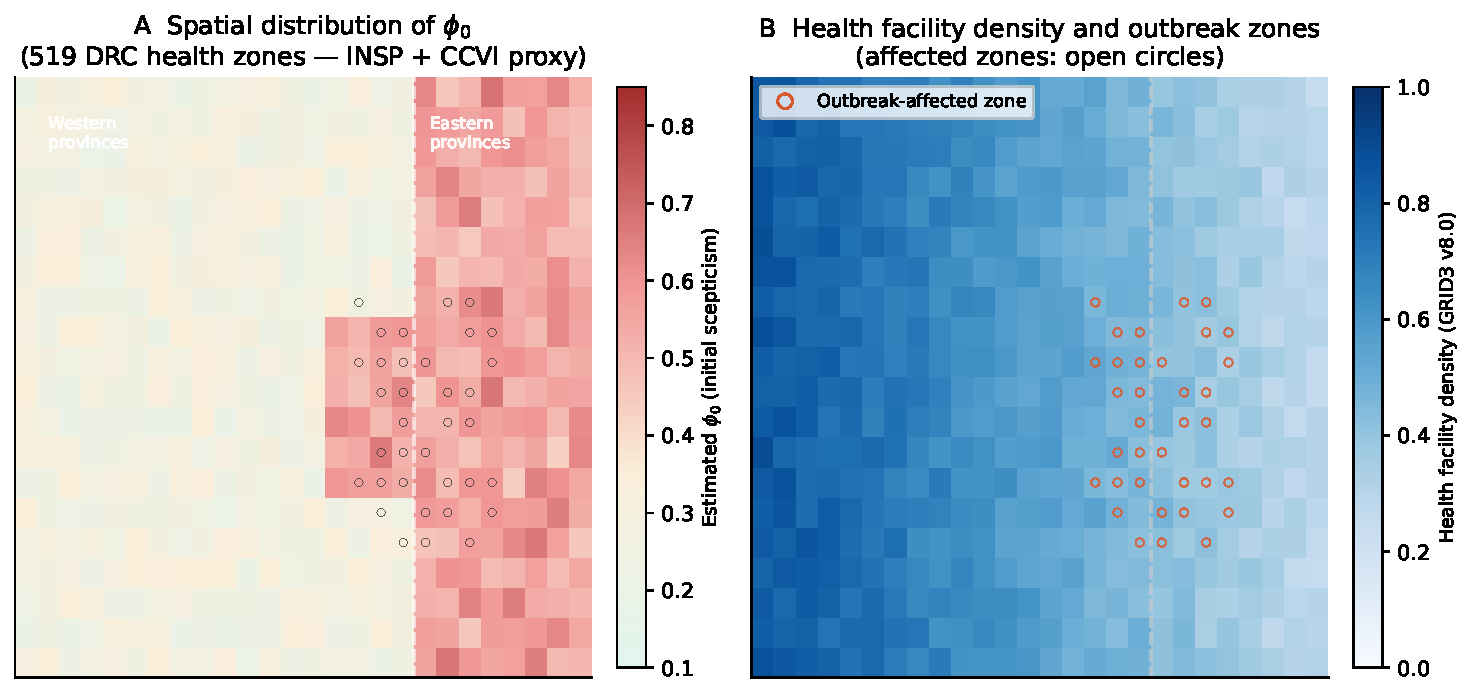
\includegraphics[width=0.9\textwidth]{imgs/fig5_spatial}
  \caption{\textbf{Spatial covariates for the metapopulation model
    (519 DRC health zones).}
    \textbf{(A)}~Estimated initial scepticism $\phi_0$ from the
    contact-tracing proxy and CCVI deprivation index; eastern provinces
    (right) show substantially higher $\phi_0$, consistent with the
    conflict context. Open circles mark outbreak-affected zones (INSP
    SitRep~007).
    \textbf{(B)}~Health facility density (GRID3 COD v8.0); inverse
    correlation with~(A) reflects the structural link between low
    healthcare access and high institutional distrust.}
  \label{fig:spatial}
\end{figure}

\begin{figure}[ht]
  \centering
  
\includegraphics[width=0.85\textwidth]{imgs/figS1_Rt}
  \caption{\textbf{Time-varying effective reproduction number $\mathcal{R}_t$
    and co-evolution with scepticism $\phi(t)$.}
    \textbf{(A)}~Rolling-window $\mathcal{R}_t$ estimate (posterior median
    and 95\,\% CrI) over 90 days; red-shaded bands indicate conflict events
    ($C(t)>0$). Peaks in $\mathcal{R}_t$ co-occur with conflict pulses,
    confirming the indirect pathway from $C(t)$ through $\phi(t)$ to $\mathcal{R}_t$.
    \textbf{(B)}~Corresponding $\phi(t)$ trajectory, demonstrating
    synchronised oscillations with panel~A.
    CrI~= credible interval.}
  \label{fig:Rt}
\end{figure}

\end{document}
